\section{Analyse de l'existant}
\subsection{Citygen}
\subsubsection{Interface et options}

L’interface est simple et facile d’usage, c'est un point and click similaire à un éditeur 3D, il y a trois modes d'édition principaux avec des options d'ajouts et de suppressions : nœuds, routes et cellules. Tout d’abord on peut créer une ville avec un affichage en temps réel avec des routes principales, en rajoutant des noeuds permettant de délimiter les périmètres d'une ville. Une fois ces noeuds reliés avec des arêtes, une cellule de ville est créer, l'affichage de bâtiments ainsi que celui des routes secondaires est automatiquement généré suite à un calcul par le système à l'aide des processus d'échantillonnage, de traçage et d'interpolation pour construire les itinéraires routiers réels à travers le terrain.\\
Les bâtiments ainsi que les routes secondaires s'adaptent donc aux changements appliqués aux routes principales.\cite{KellyLog} \\

La génération d'une ville avec Citygen représente bien la géométrie urbaine typique d'une ville moderne. Avec les options d’affichage ciblé integré, il est plus facile de voir le fonctionnement à travers les tests unitaires effectués.\\

Il existe aussi une vidéo d'utilisation démonstrative sur le site officiel du programme.\cite{video}

\subsubsection{Analyse des options et tests}

Le terrain est une image en .png ayant une perspective en 3D, on peut changer le terrain en y important notre propre image de terrain.

\begin{center}
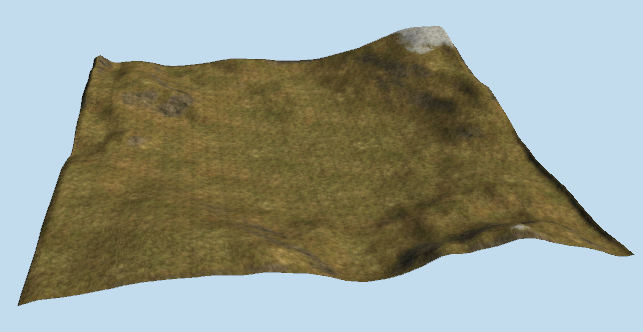
\includegraphics[height = 5 cm]{images/terrain.png}\\
\captionof{figure}{\small{Capture d'écran du terrain 3D du logiciel de base}}

\end{center}

\subsubsection{\textbf{Génération d'une route principale}}

En utilisant le bouton Node Edit puis Add Node, on délimite notre ville en posant 5 noeuds.

\begin{figure} 
\begin{minipage}[c]{.46\linewidth}
	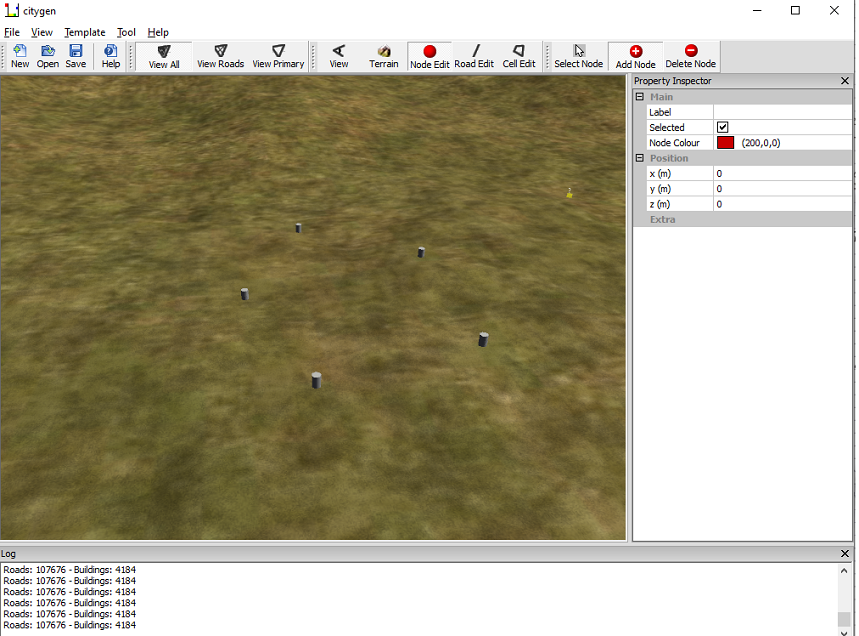
\includegraphics[height = 5 cm]{images/figure1.png}\\
	\captionof{figure}{\small{Capture d'écran personnelle du logiciel Citygen}}
\end{minipage} \hfill 
\begin{minipage}[c]{.46\linewidth}
	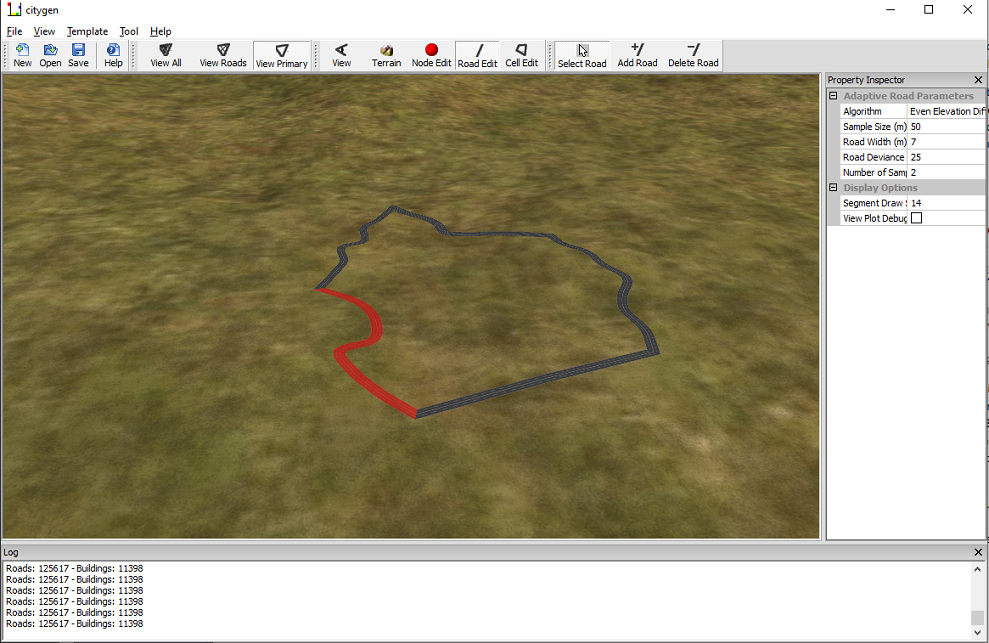
\includegraphics[height = 5 cm]{images/figure2.png}\\
	\captionof{figure}{\small{Capture d'écran personnelle du logiciel Citygen}}
\end{minipage}
\end{figure}

Une fois les noeuds reliés entre eux avec des arêtes, la cellule de ville est créée, on aperçoit la génération de nos routes principales avec des options à droite permettant aux routes principales d'être manipulées de manière interactive.

\subsubsection{\textbf{Génération d'une route secondaire}}

\begin{center}
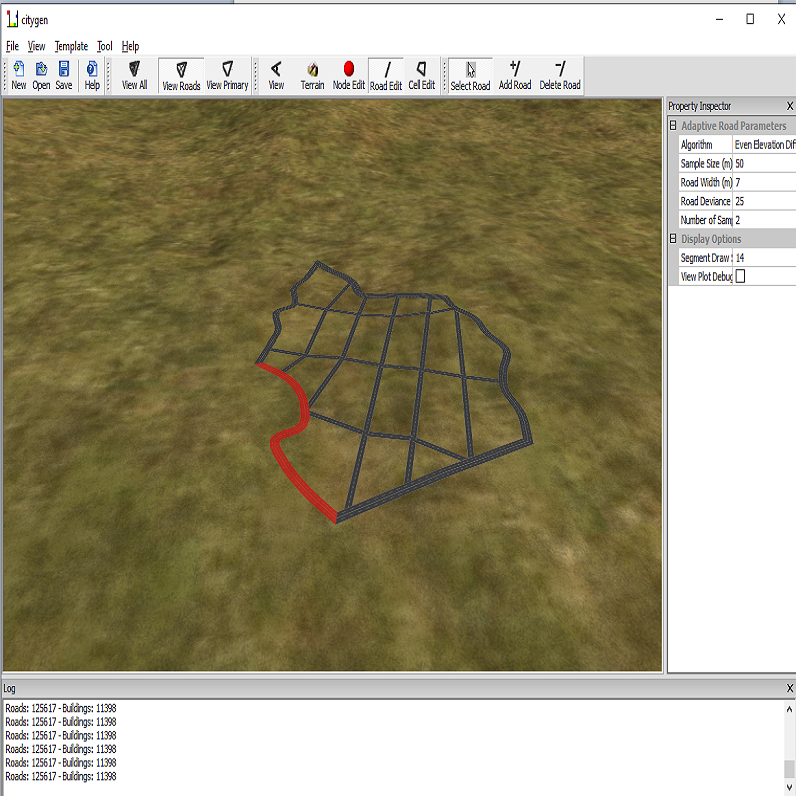
\includegraphics[height = 5 cm]{images/figure3.png}\\
\captionof{figure}{\small{Capture d'écran personnelle du logiciel Citygen}}
\end{center}
Les routes secondaires ne sont modifiables qu'en manipulant les routes principales et sont générées automatiquement à l'aide d'un algorithme basé sur la croissance.

\subsubsection{\textbf{Génération d'un bâtiment}}

Les bâtiments sont générés automatiquement grâce à un processus de lôtissements et sont également modifiables en manipulant les routes principales.
Il y a 125617 routes et 11398 bâtiments.
\newline
On peut aussi ouvrir un fichier de ville moderne (.cgx) conçu et sauvegarder le notre.

\textbf{\tab Entree : } Un fichier de ville (format .cgx)

\textbf{\tab Sortie : } Une représentation graphique d'une ville générée par le fichier
    
    
    \tab Le logiciel vérifie que le fichier d'entrée est un fichier .cgx, il y a 7383 routes et 67759 bâtiments et l'affichage est quasi-instantané.

\begin{figure} 
\begin{minipage}[c]{.46\linewidth}
	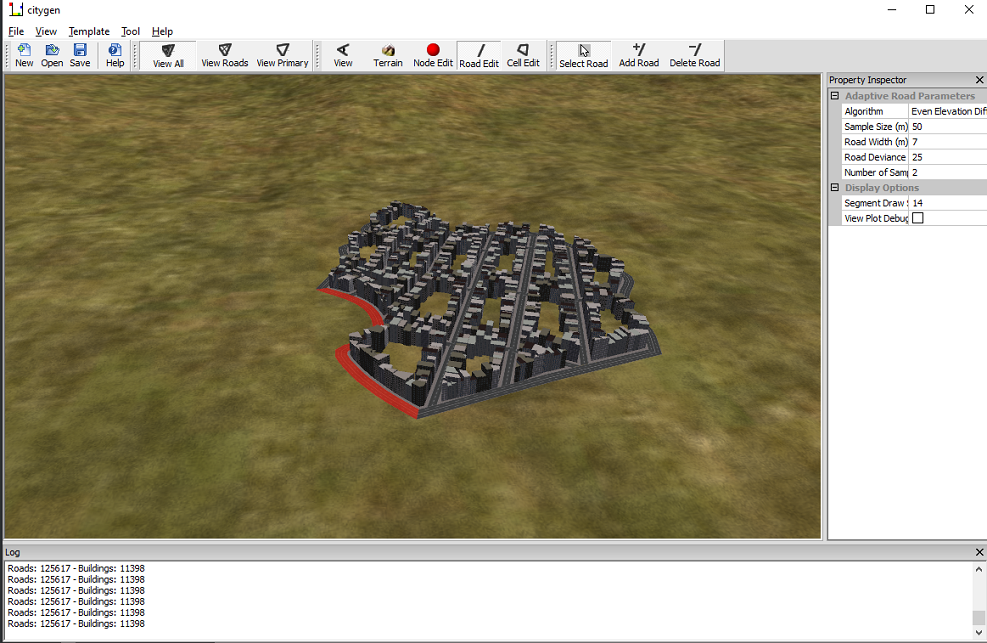
\includegraphics[height = 5 cm]{images/figure4.png}\\
	\captionof{figure}{\small{Capture d'écran personnelle du logiciel Citygen}}
\end{minipage} \hfill 
\begin{minipage}[c]{.46\linewidth}
	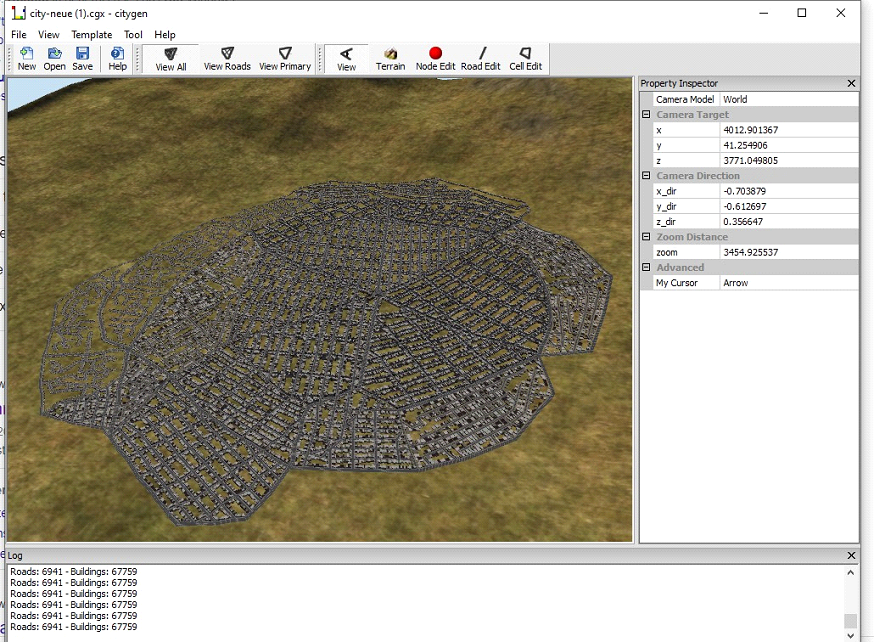
\includegraphics[height = 5 cm]{images/figure5.png}\\
	\captionof{figure}{\small{Capture d'écran personnelle de l'importation d'une ville déjà conçue}}
\end{minipage}
\end{figure}

\subsubsection{Analyse des éléments de la ville}

\subsubsection{\textbf{Les routes principales}}

\begin{center}
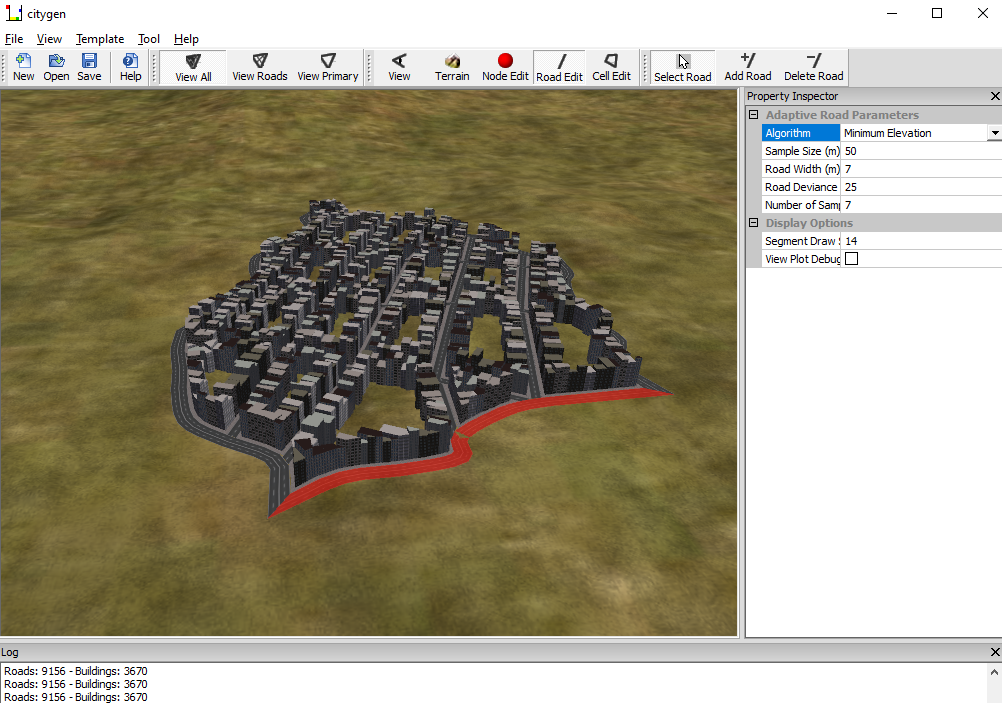
\includegraphics[height = 5 cm]{images/figure6.png}\\
\captionof{figure}{\small{Capture d'écran personnelle d'une route sélectionnée avec l'algorithme Minimum Elevation}}
\end{center}
Route avec l'algorithme Minimum Elevation :
L'échantillon avec l'altitude (Elevation) la plus basse est sélectionnée.

\subsubsection{\textbf{Les routes secondaires}}

\begin{center}
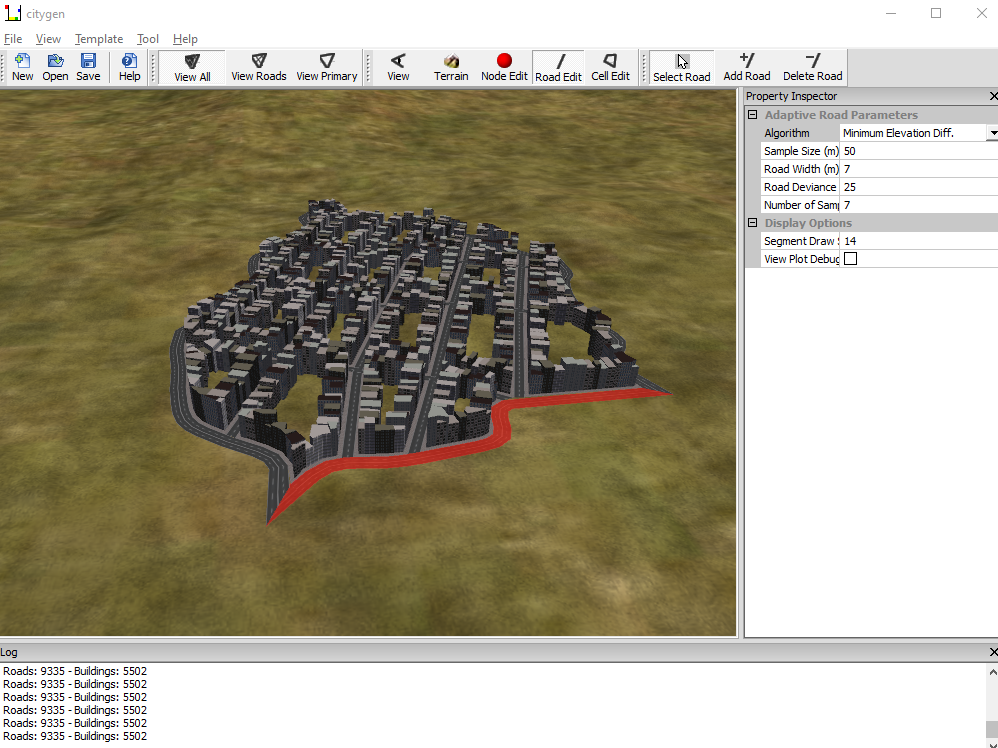
\includegraphics[height = 5 cm]{images/figure6bis1.png}\\
\captionof{figure}{\small{Capture d'écran personnelle d'une route sélectionnée avec l'algorithme Minimum Elevation Diff}}
\end{center}
Route avec l'algorithme Minimum Elevation Diff :
L'échantillon avec une altitude uniforme pour l'ensemble du segment de route.

\subsubsection{\textbf{Les bâtiments}}

\begin{center}
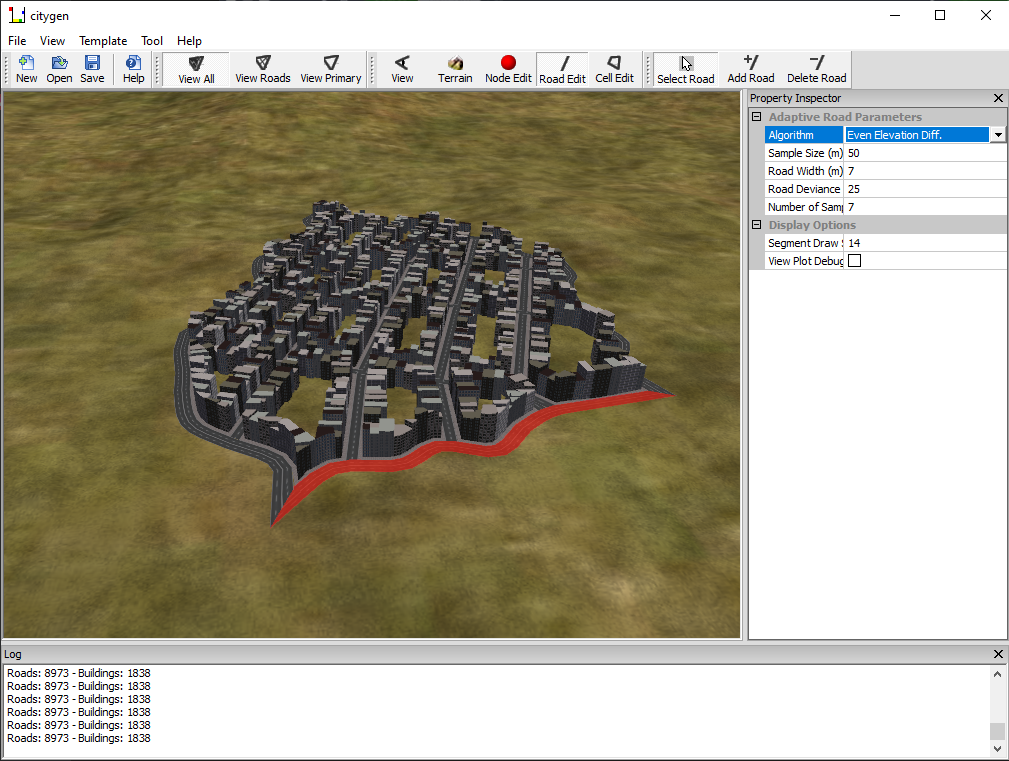
\includegraphics[height = 5 cm]{images/figure6bis2.png}\\
\captionof{figure}{\small{Capture d'écran personnelle d'une route sélectionnée avec l'algorithme Even Elevation Diff}}
\end{center}
Route avec l'algorithme Even Elevation Diff :
L'échantillon avec une altitude uniforme et plus lisse avec plus de courbes.
Le choix de routes selon une altitude est une bonne idée pour une meilleure impression d'une visualisation en 3D.

\subsubsection{Performances de Citygen}
Le logiciel crash de temps en temps quand on essaye de mettre des grandes valeurs en paramètres. Quant au temps d’affichage quand on load un fichier de carte est quasi-instantané, pareil pour la génération de routes.
\subsubsection{Compatibilite}
Le logiciel Citygen ne marche que sur Windows, une carte de ville déjà prête y est fournie pour un test initial.

\subsection{Medieval Fantasy City Generator}
\subsubsection{Interface et fonctionnement}
L'interface est également simple et facile d'usage, un point and click qui inclue, en revanche on a des raccourcis claviers pour les différentes options, le programme nous donne un résultat en 2D sous la forme d'une image où il y a plusieurs éléments de ville de style médievale , comme des citadelles, des temples, des châteaux, des bidonvilles, des fermes, une côte maritime, des rivières, des zones vertes (forêts, etc...), des routes, des murs, des arbres.. Il est possible de changer la couleur des écritures et l'ensemble des éléments de la carte grâce à un code de couleur en héxadécimal ou une configuration manuelle en HSV.

\subsubsection{Analyse des options et tests}

Il y a également plusieurs options proposées comme la génération d'une nouvelle ville aléatoire avec un nom aléatoire et des noms de districts qu'on peut ensuite modifier, soit en cliquant sur le texte directement ou bien à travers l'option Settlement, on peut également ajouter un nouveau texte directement avec l'option Landmark.\\

Il y a l'outil Warp permettant de manipuler les différentes options de générations, comme celle qui permet de modifier la taille des routes ainsi que les batîments, ajouter de l'eau, égaliser les éléments affichés, mesurer, déplacer, appliquer une rotation à la ville, il y a également une option interessante qui permet de défaire les modifications qu'on souhaite appliquées et qui n'ont pas été appliquées encore.\\

On a la possibilité d'enregistrer notre ville générée sous la forme d'une image en PNG, mais également de générer une ville sur mesure mais d'une manière aléatoire en choississant les éléments de ville possibles qu'on y souhaite intégrer, ainsi que le nombre de routes (un nombre par défaut, maximal ou bien encore pré-défini), et la taille de la ville souhaîtée (Small, Medium, Large).\\

On peut également enregistrer ou bien partager la ville générée à travers un lien permanent qu'on peut avoir sous forme d'URL, ou encore bien sous la forme d'un fichier SVG pour une perte minimale de la qualité d'image. Il y a la possibilté d'enregistrer sous la forme d'un fichier JSON pour les changements de style et de couleurs.\\

Le partage sous forme d'URL fonctionne correctement, conserve les proportions ainsi que les noms donnés, mais ne conserve pas les modifications de styles, les différentes couleurs des éléments de la ville, la taille, la police et le style des noms de villes.\\

Pour l'exportation du style il faut avoir recours au fichier JSON, mais l'import d'un fichier de style JSON ne semble pas fonctionner.
Il y a aussi une échelle représentant la distance sur la carte et sa correspondance sur le terrain, tandis que la boussole est purement  décorative (ne change pas dans le cas d'une rotation).
Il y a également une option pour un affichage plein écran \cite{medieval}
\begin{center}
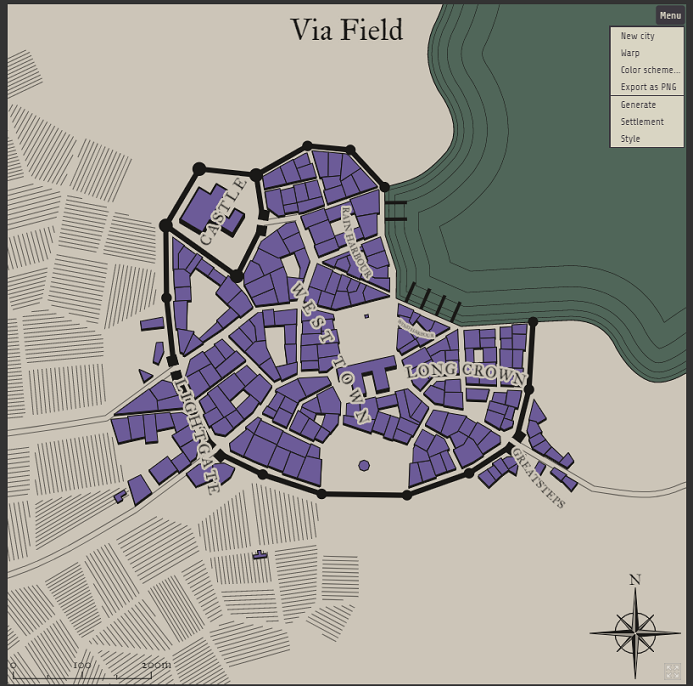
\includegraphics[height = 5 cm]{images/figure8.png}\\
\captionof{figure}{\small{Capture d'écran prise sur une machine personnelle d'une ville générée avec le programme}}
\end{center}

\subsubsection{Performances de Medieval Fantasy City Generator}

Le programme web prends un temps de moins d'une seconde quand il s'agit de générer une ville aléatoirement ou bien avec des choix pré-définis, et une à deux secondes quand il s'agit d'appliquer des modifications sur les éléments de la ville.

\subsubsection{Compatibilité}

Le programme est compatible avec la majorité des appareils nouvelles générations et donc l'ensemble des systèmes d'exploitations supportant un navigateur Web capable d'afficher du JavaScript (iOs, Android,
MacOS, GNU/Linux, Windows ...).

\subsubsection{Performances de la machine de test}

\begin{center}
  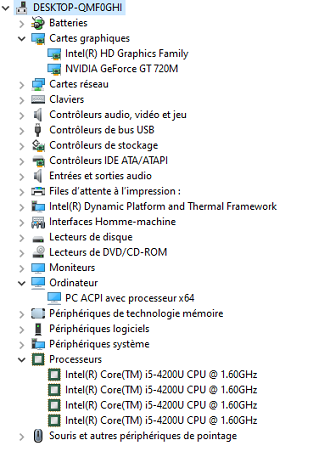
\includegraphics[height = 7 cm]{images/figure9.png}
  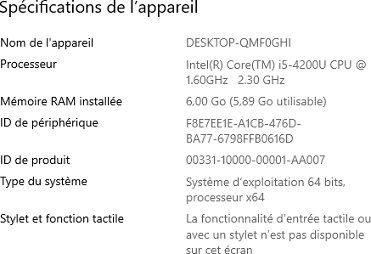
\includegraphics[height = 7 cm]{images/figure10.png}\\
  \captionof{figure}{\small{Specification de l'appareil}}
\end{center}

Ces tests et ces captures de logiciels ont été réalisées sur une machine personnelle dôtée d'un processeur x64 i5 à deux coeurs, 1.60GhZ 2.30 GHz, une Ram de 6 Go et une carte graphique NVIDIA GeForce GT 720M, une configuration plutôt moyenne qui permet de faire marcher ces logiciels existants avec de bonnes performances.

L'accessibilité ainsi que la faisabilité du projet sur une machine moyenne montre que le projet est à la fois à portée de beaucoup de monde, mais aussi réalisable d'un côté developpement.
